\documentclass[12pt]{standalone}

\usepackage{xcolor}
\usepackage[prefix=solar-]{xcolor-solarized}

\usepackage{tikz}

\begin{document}
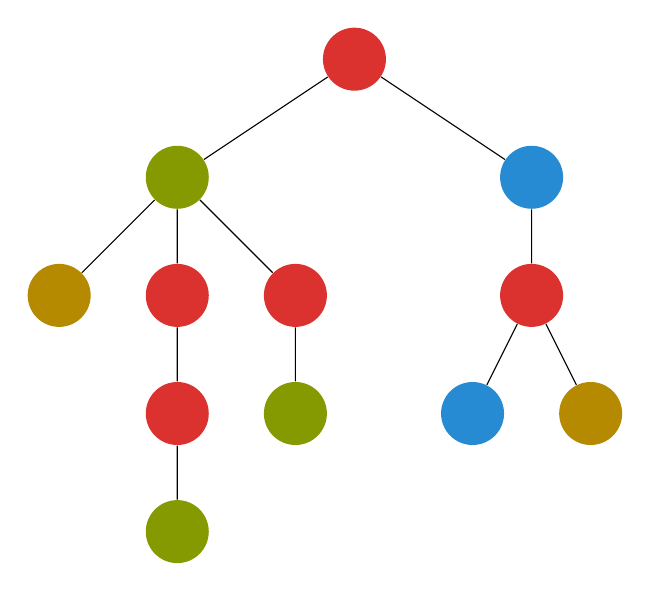
\begin{tikzpicture}[x=15mm,y=15mm]
    \begin{scope}[every node/.style={circle,fill,minimum size=8mm}]
        \node[solar-red] (A) at (0,1) {};

        \node[solar-green] (B) at (-1.5,0) {}
            child {node[solar-yellow] {}}
            child {node[solar-red] {}
                child {node[solar-red] {}
                    child {node[solar-green] {}}}}
            child {node[solar-red] {}
                child {node[solar-green] {}}};

        \node[solar-blue] (C) at (1.5,0) {}
            child {node[solar-red] {}
                child {node[solar-blue] {}}
                child {node[solar-yellow] {}}};
    \end{scope}

    \path (A) edge (B) edge (C);
\end{tikzpicture}
\end{document}
